\section*{Problem Statement}
The objective of this problem is to solve a system of linear equations
\[
  AX = b
\]
using the Jacobi Iteration method, which is an iterative approach to approximate the solution of a system of equations without direct matrix inversion.

\begin{quote}
  \textbf{NOTE}: The code can be accessed using this link: \href{https://raw.githubusercontent.com/HavokSahil/computational-techniques-assignments/refs/heads/main/assignment2/a4.m}{MATLAB}, \href{https://raw.githubusercontent.com/HavokSahil/computational-techniques-assignments/refs/heads/main/assignment2/a4.jl}{Julia}.
\end{quote}
\section*{Methodology}
The Jacobi method decomposes the coefficient matrix $A$ into a diagonal part $D$ and the remainder $Q$:
\[
  A = D - Q, \quad D = \text{diag}(A).
\]
The iteration scheme is then given by:
\[
  X^{(k+1)} = D^{-1} \big( b + Q X^{(k)} \big).
\]

The algorithm proceeds as:
\begin{enumerate}
  \item Initialize with a random guess $X^{(0)}$.
  \item For $k = 1, 2, \dots, K$:
    \[
      X^{(k+1)} = D^{-1}(b + QX^{(k)})
    \]
  \item Repeat until convergence or until the maximum number of iterations $K$ is reached.
\end{enumerate}

To assess convergence, the error norm is computed with respect to the exact solution $X_{\text{true}} = A^{-1}b$ after a varying number of iterations.

\section*{Results}
For the given system:
\[
A = \begin{bmatrix}
10 & 2 & 1 \\
2 & 20 & -2 \\
-2 & 3 & 10
\end{bmatrix}, \quad
b = \begin{bmatrix}
9 \\ -44 \\ 22
\end{bmatrix},
\]
the Jacobi iteration converges to the true solution:
\[
X = \begin{bmatrix}
1.0000 \\
-2.0000 \\
3.0000
\end{bmatrix}.
\]

The convergence behavior is shown in Figure~\ref{fig:a4}. The error decreases as the number of iterations increases, demonstrating the iterative refinement of the solution.

\begin{figure}[h!]
  \centering
  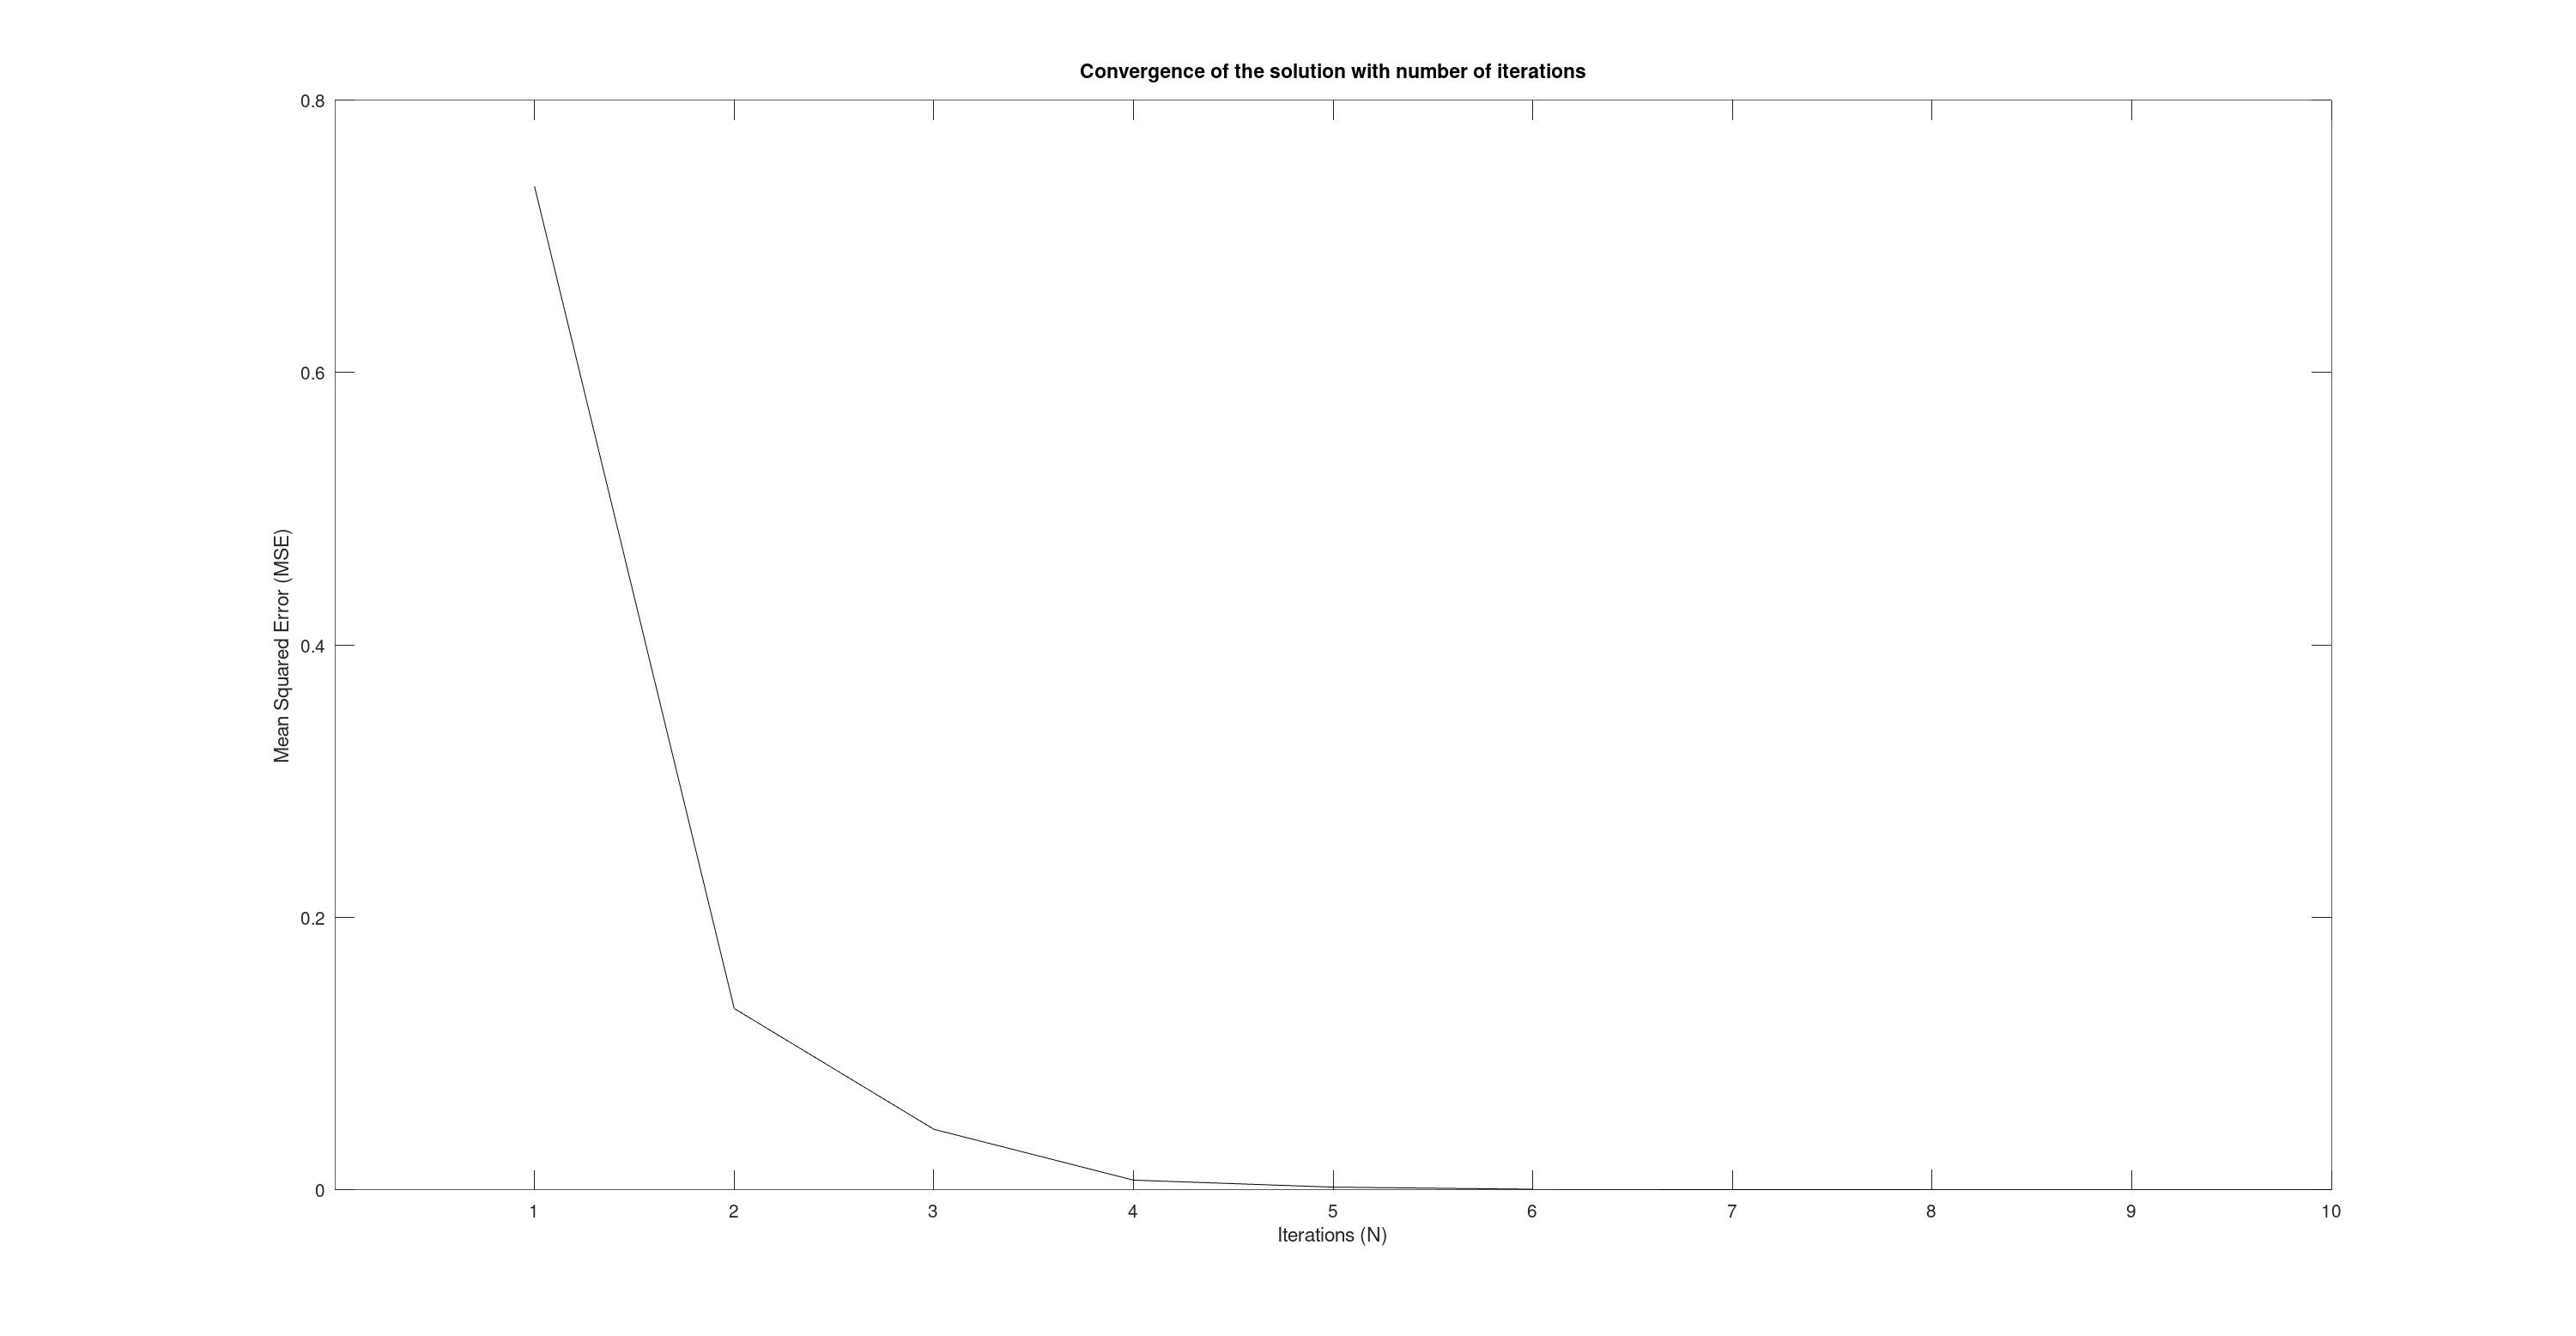
\includegraphics[width=1.0\textwidth]{a4.jpg}
  \caption{Convergence of the Jacobi iteration method. Error norm plotted against the number of iterations.}
  \label{fig:a4}
\end{figure}

\section*{Conclusion}
The Jacobi Iteration method successfully approximates the solution of the given linear system. The error decreases monotonically with iterations, illustrating convergence of the method. However, compared to direct methods like LU decomposition, Jacobi iteration requires more steps and may converge slowly depending on the properties of $A$. Its simplicity and parallelizability make it useful for large sparse systems.
